% !TeX spellcheck = cs_CZ
%---------------------------------------------------------------------------------------------------
% file fey2ch42.tex
%---------------------------------------------------------------------------------------------------
%=========================== Kapitola: Zakřivený prostor ===========================================
\setchaptertoc
\chapter{Zakřivený prostor}\label{fyz:IIchapXLII}
  \section{Zakřivené prostory se dvěma rozměry}\label{fyz:IIchapXLIIsecI}
    Podle Newtona se vše navzájem přitahuje silou, která je nepřímo úměrná druhé mocnině vzájemné 
    vzdálenosti, a tělesa reagují na síly zrychleními, která jsou silám úměrná. To jsou Newtonovy 
    zákony obecného gravitačního působení a pohybu. Jak víte, vysvětlují pohyby míčů, planet, 
    oběžnic, galaxií atd.
    
    Einstein vytvořil jinou interpretaci zákona gravitace. Podle ní prostor a čas, které dohromady 
    tvoří \textbf{časoprostor}, jsou v blízkosti velkých hmotností \emph{zakřiveny}. Pohyb těles, 
    jak jej známe, je důsledkem jejich snahy pohybovat se po „přímkách“ v zakřiveném prostoru. Je 
    to velmi, velmi, rafinovaná myšlenka, kterou chceme v této kapitole objasnit.
    
    Naše téma se skládá ze tří částí. Jedna se zabývá gravitačními jevy. Druhá obsahuje myšlenku 
    časoprostoru, kterou jsme se už zabývali. Třetí zahrnuje pojem \emph{zakřiveného časoprostoru}. 
    Na začátku všechno zjednodušíme tím, že se nebudeme starat o gravitaci a vynecháme čas-budeme 
    hovořit jen o zakřiveném prostoru. Později si všimneme i ostatních složek, ale nyní se 
    soustředíme na myšlenku zakřiveného prostoru: co se rozumí zakřiveným prostorem, nebo přesněji, 
    co se pod ním rozumí v této konkrétní Einsteinově aplikaci. I toto je obtížné v případě 
    trojrozměrného prostoru. Proto nejdříve problém ještě více zredukujeme a promluvíme si o tom, 
    co se rozumí pojmem „zakřivený prostor“ ve dvou rozměrech.

    \begin{figure}[ht!] %\ref{fyz:fig516}
      \centering
      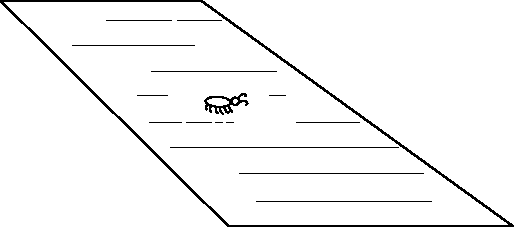
\includegraphics[width=0.7\linewidth]{fyz_fig516.pdf}
      \caption{Brouk na rovině (\cite[s.~775]{Feynman02})}
      \label{fyz:fig516}
    \end{figure}
    
    Abychom pochopili myšlenku zakřiveného prostoru ve dvou rozměrech, musíme si uvědomit omezené 
    pozorovací schopnosti obyvatele takového prostoru. Představme si brouka bez očí, který žije na 
    rovině, jak ukazuje obr. \ref{fyz:fig516}. Může se pohybovat jen po rovině a nemá možnost 
    zjistit, že lze objevit nějaký „vnější svět“. (Nemá naši představivost.) Samozřejmě, naše úvahy 
    se budou zakládat na analogii. My žijeme v trojrozměrném světě a nemáme představu, jak z něj 
    lze vyjít nějakým novým směrem; musíme si tedy pomoci analogií. Je to tak, jako bychom byli 
    brouky na rovině, ale v jiném směru by existoval prostor. Proto se nejdříve budeme zabývat 
    broukem a budeme předpokládat, že musí žít na své ploše a nemůže ji opustit.
    
    Jako jiný příklad brouka, žijícího ve dvou rozměrech, si představte takového, který žije na 
    povrchu koule. Představujeme si, že se může procházet po povrchu koule jako na obr. 
    \ref{fyz:fig517}, ale nemůže se podívat „nahoru“, ani „dolů“, ani „ven“.
    
    \begin{figure}[ht!] %\ref{fyz:fig517}
      \centering
      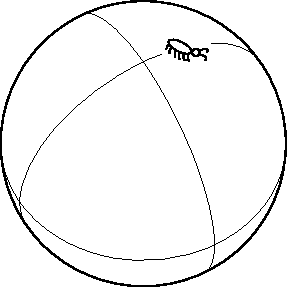
\includegraphics[width=0.5\linewidth]{fyz_fig517.pdf}
      \caption{Brouk na kouli (\cite[s.~775]{Feynman02})}
      \label{fyz:fig517}
    \end{figure}
    
    Dále si všimneme třetí bytosti.Je to opět brouk jako oba předcházející a žije na rovině jako 
    náš první brouk, ale rovina je tentokrát zvláštní. Její teplota je na různých místech různá. 
    Navíc brouk i všechna jeho pravítka jsou z látky, která se roztahuje, je-li zahřáta. Kdykoliv 
    položí své pravítko na nějaké místo, aby si něco změřil, pravítko se okamžitě roztáhne na 
    délku, která přísluší teplotě v daném místě. Kdykoliv položí nějaké těleso, sebe, pravítko, 
    trojúhelník, cokoliv, těleso se v důsledku teplotní roztažnosti zvětší. Vše je na horkých 
    místech delší než na chladných a vše má stejný koeficient teplotní roztažnosti. Domov tohoto 
    třetího brouka budeme nazývat \uv{zahřátá plotýnka} ačkoliv budeme mít na mysli speciální druh 
    takové plotýnky, která je chladná ve středu a zahřívá se směrem k okrajům (obr. 
    \ref{fyz:fig518}).
    
    \begin{figure}[ht!] %\ref{fyz:fig518}
      \centering
      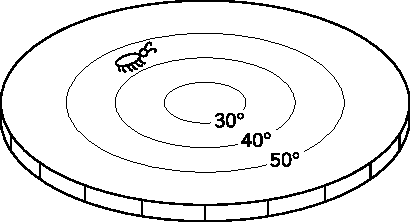
\includegraphics[width=0.7\linewidth]{fyz_fig518.pdf}
      \caption{Brouk na ohřáté desce (\cite[s.~776]{Feynman02})}
      \label{fyz:fig518}
    \end{figure}
    
    Nyní si představíme, že naši brouci začnou studovat geometrii. Ačkoliv si představujeme, že 
    jsou slepí, takže nevidí „vnější“ svět, dokáží pomocí tykadel a nohou mnoho věcí. Umí kreslit 
    čáry, vyrábět pravítka a měřit délky. Začnou od nejjednoduššího geometrického pojmu. Naučí se 
    nakreslit úsečku - nejkratší spojnici dvou bodů. Náš první brouk (viz obr. \ref{fyz:fig519}) se 
    naučí kreslit velmi pěkné čáry. Co se však stane našemu broukovi na kouli? Nakreslí svou úsečku 
    jako nejkratší - pro něj nejkratší - spojnici dvou bodů (obr. \ref{fyz:fig523}). Nám může 
    připadat jako křivka, on  se však od koule vzdálit nemůže, aby zjistil, že „ve skutečnosti“ 
    existuje i kratší úsečka. On jen ví, že vyzkouší-li ve svém světě jinou cestu, je každá delší 
    než jeho úsečka. Jeho úsečkou je tedy nejkratší oblouk mezi dvěma body. (Je to, samozřejmě, 
    oblouk tzv. hlavní kružnice.)

    \begin{figure}[ht!] %\ref{fyz:fig519}
      \centering  
      \subcaptionbox{\label{fyz:fig519a}}{\luafigure[0.5]{fyz_fig519a.pdf}}    \\
      \subcaptionbox{\label{fyz:fig519b}}{\luafigure[0.5]{fyz_fig519b.pdf}}                 
      \caption{\uv{Úsečka} v rovině a na kouli (\cite[s.~776]{Feynman02})}
      \label{fyz:fig519}
    \end{figure}  
    
    Konečně náš třetí brouk z obr. \ref{fyz:fig518} také bude kreslit „úsečky“, které nám budou 
    připadat jako křivky. Například nejkratší vzdálenost mezi \(A\) a \(B\) na obr. 
    \ref{fyz:fig521} bude podobný znázorněné křivce. Proč? Protože když se jeho křivka zakřivuje 
    směrem k teplejším částem jeho ohřáté desky, pravítka se prodlouží (z našeho vševědoucího 
    hlediska) a stačí přiložit pravítko méně krát, abychom dosáhli z \(A\) do \(B\). Pro něj je 
    čára přímá; nemá možnost vědět, že může existovat kdosi v podivném trojrozměrném světě, kdo by 
    za přímku považoval jinou čáru.
    
    \begin{figure}[ht!] %\ref{fyz:fig521}
      \centering
      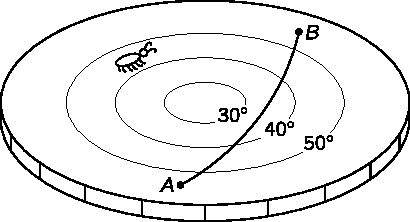
\includegraphics[width=0.7\linewidth]{fyz_fig521.pdf}
      \caption{\uv{Úsečka} na ohřáté desce (\cite[s.~776]{Feynman02})}
      \label{fyz:fig521}
    \end{figure}
    
    Myslím, že jsme pochopili, že celý náš další výklad musí vycházet z hlediska bytostí na různých 
    površích, a ne z našeho hlediska. S tímto vědomím se podíváme, jak bude vypadat zbytek jejich 
    geometrie. Předpokládejme, že všichni brouci se naučili jak nakreslit dvě přímky, které se 
    protínají pod pravým úhlem. (Můžeme zkusit vymyslet, jak by to mohli udělat.) Náš první brouk 
    (ten, co se nachází na obyčejné rovině) zjistí zajímavou věc. Vyjde-li z bodu \(A\), nakreslí 
    úsečku dlouhou \SI{100}{\cm}, pak se otočí o pravý úhel, vyznačí dalších \SI{100}{\cm}, znovu 
    se otočí o \SI{90}{\degree} a projde dalších \SI{100}{\cm}, potřetí udělá pravý úhel a nakreslí 
    čtvrtou stocentimetrovou úsečku, vrátí se do počátečního bodu, jak to znázorňuje obr. 
    \ref{fyz:fig522a}. To je vlastnost jeho světa, jedna ze skutečností jeho „geometrie".
    
    \begin{figure}[ht!] %\ref{fyz:fig522}
      \centering  
      \subcaptionbox{\label{fyz:fig522a}}{\luafigure[0.60]{fyz_fig522a.pdf}}    \\
      \subcaptionbox{\label{fyz:fig522b}}{\luafigure[0.60]{fyz_fig522b.pdf}}    \\
      \subcaptionbox{\label{fyz:fig522c}}{\luafigure[0.60]{fyz_fig522c.pdf}}              
      \caption{Čtverec, trojúhelník a kružnice v plochém prostoru (\cite[s.~777]{Feynman02}).}
      \label{fyz:fig522}
    \end{figure}     
    
    Pak objeví jinou zajímavost. Nakreslí-li trojúhelník - obrázek ze tří úseček - součet úhlů je 
    roven \SI{180}{\degree}, tj. součtu dvou pravých úhlů (obr. \ref{fyz:fig522b}).
    
    Dále objeví kružnici. Co je kružnice? Kružnici vytvoříme takto: Vyjdeme po přímkách z jediného 
    bodu mnoha směry a zakreslíte množství bodů, které mají stejnou vzdálenost od daného bodu (obr. 
    \ref{fyz:fig522c}). (Musíme geometrické pojmy pečlivě definovat, abychom dokázali udělat jejich 
    analogii v případě broukových kamarádů.) Samozřejmě, je to ekvivalentní křivce, kterou získáme 
    otočením pravítka kolem bodu. V každém případě se náš brouk naučí nakreslit kružnici. Jednoho 
    dne si pak usmyslí změřit její délku. Změří různé kružnice a zjistí pěknou zákonitost: Délka 
    kružnice je vždy součinem stejného čísla a poloměru \(r\) (což je, samozřejmě, vzdálenost od 
    středu křivky). Obvod a poloměr mají vždy stejný poměr, přibližně \num{6.283}, který nezávisí 
    na velikosti kružnice.

    \begin{figure}[ht!] %\ref{fyz:fig523}
      \centering
      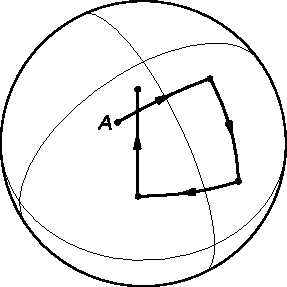
\includegraphics[width=0.5\linewidth]{fyz_fig523.pdf}
      \caption{Pokus nakreslit \uv{čtverec} na kouli
               (\cite[s.~777]{Feynman02})}
      \label{fyz:fig523}
    \end{figure}

    Nyní se podívejme, co objevili ostatní brouci v jejich geometriích. Nejdříve: co se stane, 
    pokusí-li se brouk na kouli nakreslit „čtverec“? Postupuje-li podle popsaných instrukcí, 
    zjistí, že výsledek pravděpodobně nestál za námahu. Dostane křivku jako na obr. 
    \ref{fyz:fig523}. Koncový bod \(B\) nesouhlasí s počátečním bodem \(A\). Vůbec se mu nepodaří 
    získat uzavřený obrazec. Vezměme kouli a vyzkoušejme si to. Podobná věc se přihodí i našemu 
    příteli na ohřáté desce. Zakreslí-li čtyři úsečky stejné délky (změřené pomocí jeho roztažných 
    pravítek), které svírají pravé úhly, získá obrázek znázorněný na obr. \ref{fyz:fig524}.

    \begin{figure}[ht!] %\ref{fyz:fig524}
      \centering
      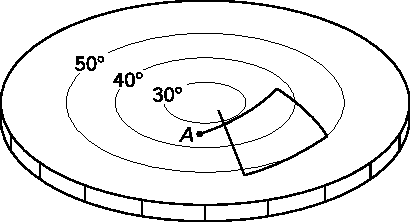
\includegraphics[width=0.7\linewidth]{fyz_fig524.pdf}
      \caption{Pokus nakreslit „čtverec“ na ohřáté desce(\cite[s.~778]{Feynman02})}
      \label{fyz:fig524}
    \end{figure}
   
    Nyní předpokládejme, že naši brouci kdysi měli své Euklidy, kteří jim řekli, jaká by „měla 
    geometrie být“, a že oni si předpovědi ověřili pomocí nepřesných měření v malém měřítku. Když 
    se pak pokusili nakreslit přesné čtverce ve velkém měřítku, zjistili, že něco není v pořádku. 
    Důležité je, že pouze na základě geometrických měření by zjistili, že je na jejich prostoru 
    něco zvláštního. Zakřivený prostor definujeme jako prostor, v němž se geometrie liší od 
    očekávání v rovině. Geometrie brouků na kouli a na ohřáté desce je geometrií v zakřiveném 
    prostoru. Zákony euklidovské geometrie tu selhávají. A vůbec není třeba se vzdálit z roviny, 
    abychom zjistili, zda svět, v němž žijeme je zakřiven. Není třeba obeplouvat zeměkouli, abychom 
    zjistili, že je kulatá. Můžeme zjistit, že žijeme na kouli, tak, že se pokusíme nakreslit 
    čtverec. Je-li čtverec velmi malý, musíme pracovat extrémně přesně, ale je-li čtverec velký, 
    měření lze udělat hrubší.

    \begin{figure}[ht!] %\ref{fyz:fig525}
      \centering
      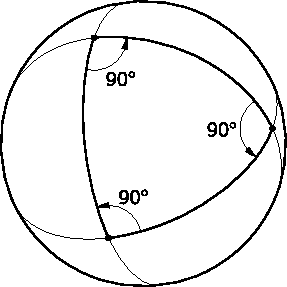
\includegraphics[width=0.7\linewidth]{fyz_fig525.pdf}
      \caption{„Trojúhelník“ na kouli může mít tři pravé úhly (\cite[s.~778]{Feynman02})}
      \label{fyz:fig525}
    \end{figure}
    
    Vezměme si případ trojúhelníka v rovině. Součet jeho úhlů je \num{180} stupňů. Náš přítel na 
    kouli může najít velmi zvláštní trojúhelníky. Může například najít trojúhelníky, které mají tři 
    pravé úhly. Opravdu! Jeden je znázorněn na ob. \ref{fyz:fig525}. Nechť náš brouk vyjde ze 
    severního pólu a nakreslí úsečku až po rovník. Potom se otočí o pravý úhel a projde další 
    úsečku stejné délky. Potom totéž provede znovu. V případě speciální délky, kterou si vybral, se 
    vrátí přesně do počátečního bodu a s první úsečkou se setká pod pravým úhlem. Je tedy 
    nepochybné, že jeho trojúhelník má tři pravé úhly, jejichž součet je \num{270} stupňů. Ukazuje 
    se, že v jeho případě je součet úhlů trojúhelníku vždy větší než \num{180} stupňů. O kolik je 
    větší (v našem speciálním případě o \SI{90}{\degree}), ve skutečnosti závisí na ploše 
    trojúhelníka. Je-li trojúhelník na kouli malý, jeho úhly se sčítají na hodnotu velmi blízkou 
    \num{180} stupňům, jen o maličko větší.
    
    \begin{figure}[ht!] %\ref{fyz:fig526}
      \centering
      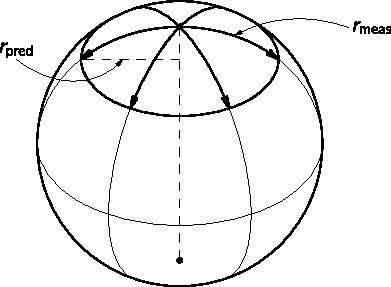
\includegraphics[width=0.7\linewidth]{fyz_fig526.pdf}
      \caption{Kružnice na kouli (\cite[s.~779]{Feynman02})}
      \label{fyz:fig526}
    \end{figure}
     
    Když se trojúhelník zvětšuje, roste i odchylka. Brouci na ohřáté desce by se svými trojúhelníky 
    měli podobné problémy.
    
    Dále se podíváme, co naši brouci zjistí o kružnici. Nakreslí kružnice a změří jejich obvody, 
    Například brouk na kouli by mohl nakreslit kružnici jako na obr. \ref{fyz:fig526}. Přitom by 
    zjistili, že obvod je menší než \(2\pi\)-násobek poloměru. (Díky moudrosti našeho 
    trojrozměrného pohledu vidíme, že to co se nazývá poloměrem, je ve skutečnosti křivka, která je 
    delší než skutečný poloměr kružnice.) Nechť má brouk na kouli prostudovanou euklidovskou 
    geometrii a rozhodne se předpovědět poloměr kružnice tak, že vydělí obvod \(C\) číslem \(2\pi\),
    \begin{equation}\label{fyz:eq528}
      r_{\text{přep}} = \dfrac{C}{2\pi}
    \end{equation}
    
    Pak zjistí, že naměřený poloměr je větší než předpovězený. Aby se s tím nějak vyrovnal, může 
    rozdíl definovat jako „nadbytečný poloměr"
    \begin{equation}\label{fyz:eq529}
      r_{\text{naměř}} - r_{\text{přep}} = r_{\text{nadb}}
    \end{equation}
    a zkoumat, jak nadbytečný poloměr závisí na velikosti kružnice. 
    
    \begin{figure}[ht!] %\ref{fyz:fig527}
      \centering
      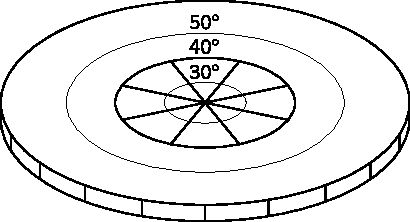
\includegraphics[width=0.7\linewidth]{fyz_fig527.pdf}
      \caption{Kružnice na ohřáté desce
               (\cite[s.~779]{Feynman02})}
      \label{fyz:fig527}
    \end{figure}
    
    Náš brouk na ohřátě desce by objevil podobný jev. Nechť má nakreslit kružnici se středem v 
    chladném bodě desky (obr. \ref{fyz:fig527}). Kdybychom sledovali, jako kreslí kružnici, 
    zjistili bychom, že jeho pravítka jsou blízko středu kratší a prodlužují se směrem od středu, 
    ačkoliv to brouk neví. Když pak měří obvod, jeho pravítko je po celou dobu dlouhé, takže také 
    zjistí, že změřený poloměr je větší než předpovězený, \(C/2\pi\). Brouk na ohřáté desce také 
    objeví „efekt nadbytečného poloměru“. A znovu velikost efektu závisí na poloměru kružnice.
    
    Zakřivený prostor budeme \emph{definovat} jako prostor, v němž se vyskytují tyto typy 
    geometrických chyb: Součet úhlů trojúhelníka se liší od \num{180} stupňů; obvod kružnice dělený 
    číslem \(2\pi\) není roven poloměru; návod na nakreslení čtverce nevede k uzavřenému obrazci. 
    Můžete si vymyslet i jiné.
    
    Uvedli jsme dva různé příklady zakřiveného prostoru: povrch koule a ohřátou desku. Je však 
    zajímavé, že zvolíme-li vhodně způsob, jak se na ohřáté desce mění teplota v závislosti na 
    vzdálenosti, budou obě geometrie úplně stejné. Je to zábavné. Můžeme dosáhnout toho, aby brouk 
    na ohřáté desce dostával přesně stejné výsledky jako brouk na kouli. Předpokládáme-li, že délka 
    pravítek (jako funkce teploty) je úměrná jedné plus konstanta krát druhá mocnina vzdálenosti od 
    počátku, zjistíte, že geometrie ohřáté desky je ve všech podrobnostech přesně stejná jako 
    geometrie koule\footnote{S výjimkou bodu v nekonečnu.}. 
    
    Samozřejmě existují i jiné geometrie. Mohli bychom se zeptat, jaká je geometrie brouka, který 
    žije na hrušce, tj. na povrchu, který má větší zakřivení na jednom místě a menší na jiném, 
    takže přebytek úhlů v trojúhelníku je větší, když brouk nakreslí malý trojúhelník v jedné části 
    svého světa, než když jej nakreslí v jiné. Jinými slovy, křivost prostoru se může od místa k 
    místu měnit. To je jen zobecnění myšlenky zakřiveného prostoru. Totéž lze imitovat i vhodným 
    rozdělením teploty na ohřáté desce. 
    
    \begin{figure}[ht!] %\ref{fyz:fig528}
      \centering
      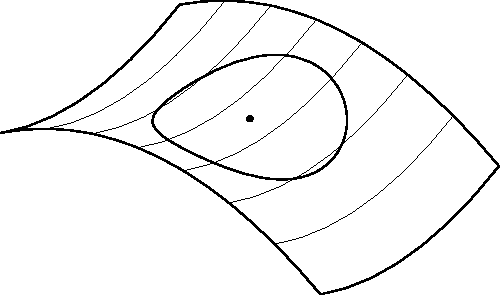
\includegraphics[width=0.7\linewidth]{fyz_fig528.pdf}
      \caption{\uv{Kružnice} na sedlovém povrchu
               (\cite[s.~780]{Feynman02})}
      \label{fyz:fig528}
    \end{figure}
  
    Také je třeba poznamenat, že výsledky by mohly vyjít i s opačným znaménkem. Mohli bychom 
    například zjistit, že všechny trojúhelníky, když jsou velmi velké, mají součet úhlů menší než 
    \num{180} stupňů. Možná že to zní neuvěřitelně, ale není to vůbec tak. Za prvé, mohli bychom 
    mít ohřátou desku, jejíž teplota se vzdáleností od středu klesá. Pak by všechny pozorované 
    efekty měly opačné znaménko. Můžeme toho však dosáhnouti čistě geometricky, podíváme-li se na 
    dvojrozměrnou geometrii sedlového povrchu. Představte si sedlovou plochu jako na obr. 
    \ref{fyz:fig528}. Nakresleme na ní „kružnici“ definovanou jako množinu bodů. které mají od 
    středu stejnou vzdálenost. Tato kružnice je křivka, která po povrchu osciluje a vytváří 
    vroubkovaný okraj. Její obvod je proto větší než očekávaných \(2\pi r\). Takže \(C/2\pi\) je 
    nyní menší než \(r\) a nadbytečný  poloměr je záporný. 
    
    Koule a hrušky apod. jsou všechno plochy s kladnou křivostí; ostatní se nazývají plochy se 
    zápornou křivostí. Obecně dvojrozměrný svět bude mít křivost, která se mění od místa k místu a 
    může být někde kladná a jinde záporná. Pod zakřiveným prostorem obecně chápeme takový prostor, 
    v němž jsou zákony euklidovské geometrie porušeny, ať už je odchylka kladného nebo záporného 
    znaménka. Velikost křivosti (definovaná, řekněme, pomocí nadbytečného poloměru) se může od 
    místa k místu měnit.

    \begin{figure}[ht!] %\ref{fyz:fig529}
      \centering
      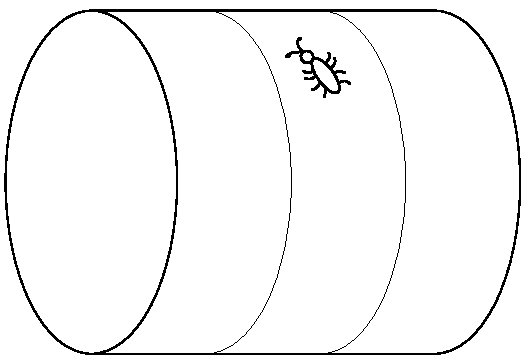
\includegraphics[width=0.7\linewidth]{fyz_fig529.pdf}
      \caption{Dvojrozměrný prostor jehož vnitřní křivost je nulová
               (\cite[s.~781]{Feynman02})}
      \label{fyz:fig529}
    \end{figure}
  
    Ještě poznamenejme, že podle naší definice křivosti není válec kupodivu zakřiven. Kdyby brouk 
    žil na povrchu válce (obr. \ref{fyz:fig527}), zjistil by, že trojúhelníky, čtverce a kruhy, by 
    se chovaly jako v rovině. O tom se lze snadno přesvědčit, představíme-li si, jak by jednotlivé 
    obrazce vypadaly, kdybychom válec rozvinuli do roviny. Pak všechny geometrické obrazce přesně 
    korespondují s tím, co máme v rovině. Pro brouka na válci (předpokládáme, že jej neobejde 
    dokola, ale provádí jen lokální měření) neexistuje způsob, jak zjistit, že je jeho prostor 
    zakřiven. V našem technickém smyslu není jeho prostor zakřiven. Veličina, o níž chceme hovořit, 
    se přesněji nazývá \textbf{vnitřní křivost}, tj. křivost, kterou můžeme objevit na základě 
    měření v lokální oblasti prostoru. (Válec má \emph{nulovou vnitřní křivost}.) Právě v takovém 
    smyslu je třeba chápat Einsteinovo tvrzení, že náš prostor je zakřiven. My jsme však definovali 
    zakřivený prostor pouze ve dvou rozměrech, musíme postoupit dále a podívat se, jaký smysl by 
    tento pojem mohl mít ve třech rozměrech.
    
  \section{Křivost v trojrozměrném prostoru}\label{fyz:IIchapXLIIsecII}
    My žijeme v trojrozměrném prostoru, a proto budeme nyní zvažovat myšlenku, že je náš prostor 
    zakřiven. Můžeme namítnout: „Ale jak si dokážeme představit, že je prostor v nějakém směru 
    zakřiven?“ Pravda, prostor zakřivený v nějakém směru si představit neumíme, neboť naše 
    představivost není dostatečná. (Možná, že je dobře, že si neumíme představit příliš mnoho věcí, 
    takže se alespoň neodtrhneme od reálného světa). Ale křivost můžeme definovat, aniž bychom z 
    našeho trojrozměrného světa vyšli. To, o čem jsme hovořili ve dvou rozměrech, bylo jen 
    rozcvičkou na to, abychom mohli zavést definici křivosti, která nevyžaduje náš „pohled zvenku“.
    
    To, zda náš svět zakřiven je nebo není, můžeme určit způsobem, který je analogický tomu, co 
    používali naši džentlmeni na kouli nebo na ohřáté desce. Možná, že nedokážeme rozlišit dva 
    takové případy, ale jistě můžeme zjistit rozdíl mezi těmito případy a plochým, nezakřiveným 
    prostorem. Dokonce velmi snadno. Nakreslíme trojúhelník a změříme úhly. Nebo vytvoříme velkou 
    kružnici a změříme její obvod a poloměr. Nebo zkusíme vytvořit přesné čtverce, případně 
    krychli. V každém případě zkoumáme, zda platí zákony geometrie. Jestliže neplatí, prohlásíme 
    náš prostor za zakřivený. Nakreslíme-li velký trojúhelník a zjistíme, že součet jeho úhlů 
    překračuje \num{180} stupňů, můžeme říci, že náš prostor je zakřiven. Není-li změřený poloměr 
    kružnice roven jejímu obvodu dělenému číslem \(2\pi\), můžeme prohlásit, že náš prostor je 
    zakřiven.
    
    Jistě si všimneme, že situace ve třech rozměrech může být mnohem složitější než ve dvou. Na 
    libovolném místě ve dvou rozměrech má křivost určitou velikost. Ale ve třech rozměrech může mít 
    křivost několik složek. Nakreslíme-li trojúhelník v nějaké rovině, výsledek může být jiný, než 
    když orientujeme rovinu trojúhelníka jiným způsobem. Nebo vezměme jako příklad kružnici. 
    Představte si, že nakreslíme kružnici, změříme její poloměr a zjistíme, že se neshoduje s 
    \(C/2\pi\), takže tu je nějaký nadbytečný poloměr. Pak nakreslíme jinou kružnici pod pravým 
    úhlem (obr. \ref{fyz:fig530}). Není důvod, proč by nadbytek měl být stejný v případě obou 
    kružnic. Ve skutečnosti v případě kružnice v jedné rovině může být nadbytek kladný a ve druhé 
    rovině záporný (úbytek).
    
    \begin{figure}[ht!] %\ref{fyz:fig530}
      \centering
      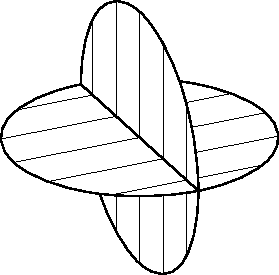
\includegraphics[width=0.5\linewidth]{fyz_fig530.pdf}
      \caption{Nadbytečný poloměr může být různý u kružnic s různými orientacemi      
               (\cite[s.~782]{Feynman02})}
      \label{fyz:fig530}
    \end{figure}
    
    Možná, že přemýšlíme o lepším nápadu: nemůžeme se zbavit všech složek tak, že ve třech 
    rozměrech použijeme kouli? Povrch koule můžeme definovat jako množinu bodů, které jsou od 
    daného bodu v prostoru stejně vzdáleny. Velikost povrchu pak můžeme změřit tak, že na ni 
    položíme jemnou pravoúhlou mřížku a sečteme všechny malé plošky. Podle Euklida má být celková 
    plocha \(S\) rovna \(4\pi\) krát druhá mocnina poloměru; „předpovídaný“ poloměr tedy můžeme 
    definovat jako \(\sqrt{S/4\pi}\). Poloměr však můžeme změřit také přímo tak, že provrtáme díru 
    do středu a změříme jeho vzdálenost. Opět můžeme od změřeného poloměru odečíst předpovídaný 
    poloměr a rozdíl nazvat nadbytkem poloměru:
    \begin{equation*}
      r_{\text{nadb}} = r_{\text{naměř}} -\left(\dfrac{\text{změřený povrch}}{4\pi}\right)^{1/2},
    \end{equation*}
    což by mohlo být dobrou mírou křivosti. Má tu velkou výhodu, že nezávisí na tom, jak 
    zorientujeme trojúhelník nebo kruh.
    
    Ale nadbytečný poloměr koule má i nevýhodu: necharakterizuje prostor úplně. Udává pouze 
    \emph{střední křivost} trojrozměrného světa, protože průměruje přes různé křivosti. Jelikož je 
    to jen průměr, neřeší úplně problém, jaká je geometrie prostoru. Známe-li pouze toto číslo, 
    nemůžeme předpovědět všechny vlastnosti geometrie prostoru, neboť nedokážeme říci co se stane s 
    kružnicemi, které mají různou orientaci. Úplná definice vyžaduje zadání šesti hodnot křivosti v 
    každém bodě. Matematici samozřejmě vědí, jak tato čísla vypočítat. Jednou si v matematické 
    knize můžeme přečíst, jak je všechny zapsat v elegantním a dokonalém tvaru, ale nejdříve je 
    lepší zhruba pochopit, o čem to vlastně budeme psát. Proto, co je naším cílem v naší kapitole, 
    většinou vystačíme se střední křivostí\footnote{Pro úplnost je třeba zmínit ještě jednu 
    okolnost. Jestliže chceme přenést model zakřiveného prostoru jako ohřátou desku do tří rozměrů, 
    musíme si představit, že délka pravítka závisí nejen na místě, ale i na orientaci, kterou má 
    když jej přiložíme. Je to zobecnění jednoduchého případu, kdy délka pravítka závisí jen na 
    místě, ale je stejná jestliže má směr ze severu na jih, z východu na západ, nebo shora dolů. 
    Toto zobecnění je nevyhnutelné, chceme-li pomocí tohoto modelu reprezentovat trojrozměrný 
    prostor s libovolnou geometrií, ačkoliv to shodou okolností nebylo třeba ve dvou rozměrech.}.

  \section{Náš prostor je zakřiven}\label{fyz:IIchapXLIIsecIII}
    Nyní přichází na řadu nejdůležitější otázka. Je pravda, že náš fyzikální trojrozměrný svět, v 
    němž žijeme je opravdu zakřiven? Od okamžiku, kdy mají lidé dost představivosti, aby si 
    uvědomili, že prostor může být zakřiven, je lidský duch zvědavý, zda je skutečný svět zakřiven 
    nebo ne. Mnozí uskutečnili přímá geometrická měření, ale nezjistili žádné odchylky. Na druhou 
    stranu, na základě úvah o gravitaci objevil Einstein, že prostor je \emph{opravdu} zakřiven. 
    Řekneme si, jaký je Einsteinův zákon pro hodnotu křivosti, a také něco o tom, jak k němu dospěl.
    
    Einstein zjistil, že prostor je zakřiven a hmota je zdrojem křivosti. (Hmota je také zdrojem 
    gravitace, takže gravitace souvisí s křivostí, ale k tomu se ještě v této kapitole vrátíme.) 
    Předpokládejme, abychom si problém zjednodušili, že hmota je spojitě rozložena s určitou 
    hustotou, která se však podle potřeby může od místa k místu měnit\footnote{Nikdo (dokonce ani 
    Einstein) neví, jak postupovat, je-li hmota soustředěna do bodů}. Einsteinovo pravidlo pro 
    výpočet křivosti je následující. Máme-li oblast prostoru, v níž se nachází hmota, a v ní 
    vybereme dostatečně malou kouli, takže hustota hmoty \(\varrho\) v ní je v podstatě konstantní, 
    je \emph{nadbytečný poloměr} koule úměrný množství hmoty v kouli. Podle definice nadbytečného 
    poloměru platí
    \begin{equation}\label{fyz:eq530}
      \text{nadbytečný poloměr } = \sqrt{\dfrac{S}{4\pi}} - r_\text{naměř} 
                                 = \dfrac{\varkappa}{3c^2}\cdot M.
    \end{equation}
    kde \(\varkappa\) je \emph{Newtonova gravitační konstanta}, \(c\) je \emph{rychlost světla} a 
    \(M=4\pi\varrho r^3/3\) je hmotnost látky uvnitř koule. To je Einsteinův vztah pro 
    \textbf{střední křivost prostoru}. 
    
    Vezměme si jako příklad naší Zemi a zapomeňme, že její hustota se od bodu k bodu mění, abychom 
    nemuseli počítat žádné integrály. Předpokládejme, že bychom její povrch změřili velmi pečlivě, 
    a pak vykopali díru do středu a změřili její poloměr. Z velikosti povrchu bychom mohli 
    vypočítat předpovídaný poloměr tak, že bychom povrch brali jako \(4\pi r^2\). Pokud bychom 
    porovnali předpovídaný poloměr se skutečným, zjistili bychom, že skutečný poloměr převyšuje 
    předpovídaný poloměr o hodnotu, kterou udává vztah (\ref{fyz:eq530}). Konstanta 
    \(\varkappa/3c^2\) 
    je rovna asi \SI{2.5e-28}{\m\per\kg}, takže na každý kilogram látky, je odchylka naměřeného 
    poloměru \SI{2.5e-28}{\m}. Dosadíme-li hmotnost Země, která je přibližně \SI{6e24}{\kg} vyjde, 
    že zemský poloměr je asi o \SI{1.5}{\mm} větší, než by měl odpovídat velikosti jejího 
    povrchu\footnote{Přibližně, neboť hustota není nezávislá na poloměru, jak jsme předpokládali.}. 
    Pokud bychom stejný výpočet zopakovali pro Slunce, zjistili bychom, že poloměr Slunce je o půl 
    kilometru větší, než by měl být. 
    
    Všimněme si, že zákon říká, že \emph{střední} křivost nad povrchem země je nulová. To však 
    neznamená že všechny složky křivosti jsou nulové. I nad Zemí může být - a ve skutečnosti je - 
    určité zakřivení. V případě kružnice v rovině bude existovat nadbytečný poloměr jednoho 
    znaménka při jistých orientacích roviny a opačného znaménka při jiných. Pouze průměr přes kouli 
    vychází nulový, když se \emph{uvnitř} nenachází žádná látka. Shodou okolností se ukazuje, že 
    existuje vztah mezi různými složkami křivosti a \emph{změnami} průměrné křivosti od místa k 
    místu. Tudíž známe-li průměrnou křivost v celém prostoru můžete detailně vypočítat křivost v 
    každém bodě. Střední křivost nad zemí se mění s výškou, takže i tam je prostor zakřiven. A 
    právě toto zakřivení se nám jeví jako gravitační síla. 
    
    Představme si brouka na rovině. Nechť na povrchu roviny existují drobné „puchýřky“. Kdykoliv 
    brouk narazí na „puchýřek“ usoudí, že jeho prostor má malou lokální oblast zakřivení. Něco 
    podobného máme ve třech rozměrech. Všude, kde se nacházejí shluky látky, má náš trojrozměrný 
    prostor lokální zakřivení - jakýsi trojrozměrný „puchýřek“. 
    
    Vytvoříme-li na rovině mnoho hrbolů, může být jejich výsledkem vedle všech „puchýřků“ i 
    globální křivost - prostor může vypadat jako koule. Bylo by zajímavé vědět, zda má náš prostor 
    takovou výslednou průměrnou křivost, jakož i lokální „puchýřky“ v důsledku shluků hmoty, jakými 
    jsou například Země a Slunce. Astrofyzikové hledají odpověď na tuto otázku na základě měření 
    galaxií ve velkých vzdálenostech. Například, liší-li se počet galaxií, který vidíme v kulové 
    slupce ve velké vzdálenosti, od našich očekávání na základě velikost poloměru slupky, máme míru 
    nadbytečného poloměru obrovské koule. Existuje naděje, že na základě takovýchto měření můžeme 
    zjistit, je-li náš vesmír jako celek v průměru plochý nebo zakřivený, zda je „uzavřený“ (jako 
    koule) nebo „otevřený“ (jako rovina). Možná, že jsme něco slyšeli o debatách, které se na toto 
    téma vedou. Diskutuje se velmi, neboť astronomická měření jsou stále ještě zcela nekonkluzivní; 
    experimentální údaje nejsou dost přesné, aby poskytly definitivní odpověď. Bohužel, nemáme ani 
    nejmenší představu o tom, jaká je globální křivost našeho Vesmíru.
    
  \section{Geometrie v časoprostoru}\label{fyz:IIchapXLIIsecIV}
    Nyní musíme něco říci o čase. Jak víme ze speciální teorie relativity, měření v prostoru a 
    měření v čase navzájem souvisí. A bylo by trochu bláznivé, kdyby se něco dělo s prostorem, 
    přičemž čas by v tom nehrál určitou úlohu. Pamatujeme si, že měření času závisí na rychlosti, 
    jakou se pohybujeme. Například pozorujeme-li chlapíka, který kolem nás proletí v raketě, 
    vidíme, že u něj vše probíhá pomaleji než u nás. Řekněme, že se vydá na cestu a vrátí se 
    \emph{podle našich hodin} přesně za \num{100} sekund; jeho hodiny mohou ukazovat, že byl pryč 
    jen \num{95} sekund. Ve srovnání s našimi běžely jeho hodiny, jakž i jiné procesy, např. údery 
    srdce, pomaleji.
    
    Všimněme si zajímavého problému. Předpokládejme, že vy jste ten chlapík v raketě. Požádáme vás, 
    abyste vystartovali na daný signál a vrátili se do výchozího místa přesně včas, abyste stihli 
    další signál - řekněme přesně o 100 sekund později podle našich hodin. A také od vás chceme, 
    abyste výlet uskutečnili tak, aby vaše hodiny ukazovaly co nejdelší \emph{uplynulý} čas. Jak se 
    máte pohybovat? Měli byste zůstat stát. Pohnete-li se, vaše hodiny budou ukazovat po návratu 
    méně než \num{100} sekund. 
    
    Ale předpokládejme, že úlohu trochu změníme. Požádáme vás, abyste vyšli z bodu \(A\) na daný 
    signál a dorazili do bodu \(B\) (oba body se vůči vám nepohybují), a to tak, že se vrátíte 
    přesně v okamžiku druhého signálu (řekněme o \num{100} sekund později podle našich nehybných 
    hodin). A opět se po vás chce, abyste výlet uskutečnili tak, že po návratu budou vaše hodinky 
    ukazovat co nejvyšší hodnotu. Jak byste to udělali? Pro jakou trajektorii a jaký jízdní řád 
    budou vaše hodiny ukazovat při příchodu největší uplynulý čas? Odpověď je, že z vašeho hlediska 
    bude výlet nejdelší, uskutečníte-li ho stálou rychlostí po přímce. Důvod je ten, že každý pohyb 
    navíc a každý vzrůst rychlosti zpomalí vaše hodiny. (Jelikož časové rozdíly závisejí na druhé 
    mocnině rychlosti, to, co ztratíte příliš rychlým pohybem na jednom místě, nikdy nedoženete 
    velmi pomalým pohybem na místě jiném.)
     
    Motiv celé této diskuze spočívá v tom, že tento nápad můžeme využít k definici úsečky v 
    časoprostoru. Analogem prostorové úsečky v časoprostoru je \emph{pohyb} konstantní rychlostí v 
    konstantním směru. 
    
    Křivce s nejmenší délkou v prostoru neodpovídá v časoprostoru dráha s nejkratším, ale s 
    \emph{nejdelším} časem, v důsledku zábavných věcí, které se dějí se znaménky časových členů v 
    teorii relativity. Pohyb „po přímce" - analog „konstantní rychlostí na přímce" -je tedy ten 
    pohyb, který přenese hodiny z jednoho místa v jednom čase na jiné místo v jiném čase tak, že 
    údaj na hodinách ukáže nejdelší uplynulý čas. To bude naše definice analogu úsečky v 
    časoprostoru.
    
  \section{Gravitace a princip ekvivalence}\label{fyz:IIchapXLIIsecV}
    Jsme připraveni přejít k zákonům gravitace. Einstein usilovalo vytvoření teorie gravitace, jež 
    by byla ve shodě s teorií relativity, kterou vytvořil dříve. Snažil se marně do té doby, než se 
    zachytil principu, který jej dovedl ke správným zákonům. Tento princip je založen na myšlence, 
    že padá-li nějaký předmět volným pádem, vše se v něm zdá být ve stavu beztíže. Například 
    družice na oběžné dráze padá volně v poli zemské přitažlivosti a proto se v něm astronaut cítí 
    bez tíže. Tato myšlenka, zformulovaná podstatně přesněji, se nazývá \textbf{Einsteinův princip 
    ekvivalence}. Souvisí se skutečností, že všechna tělesa padají se stejným zrychlením bez ohledu 
    na jejich hmotnost a na to, z čeho se skládají. Pohybuje-li se raketa bez motorů, tj. vlastně 
    volným pádem, a v ní se nachází člověk, zákony, které řídí pád člověka i rakety jsou stejné. 
    Přemístí-li se do středu rakety, zůstane tam. \emph{Vzhledem k raketě} nepadá. To máme na 
    mysli, když říkáme, že je v beztížném stavu.
    
    Dále si představte, že jste v raketě, která se pohybuje se zrychlením. Se zrychlením vzhledem k 
    čemu? Řekněme, že její motory jsou zapnuty a vytvářejí tah, takže raketa nepluje volným pádem. 
    Také si představte, že  jste daleko v prázdném prostoru, takže na raketu nepůsobí prakticky 
    žádné gravitační síly. Je-li zrychlení rakety právě \(g\) dokážete stát na její podlaze a 
    cítíte svou normální tíhu. Pustíte-li míč, bude padat na podlahu. Proč? Protože raketa se 
    zrychluje směrem nahoru, ale míč necítí žádné síly, a proto nezrychluje a setrvává. Uvnitř 
    rakety se zdá, že míč má zrychlení \(g\) směrem dolů.
    
    Tuto situaci porovnejme s tím, co se děje v raketě, která klidně odpočívá na povrchu Země. 
    \emph{Vše je stejné!} Přitahuje nás to k Zemi, míč padá se zrychlením \(g\) atd. Skutečně, jak 
    můžete uvnitř rakety usoudit, zda sedíte na Zemi, nebo se zrychlujete ve volném prostoru? Podle 
    Einsteinova principu ekvivalence neexistuje způsob jak rozlišit obě situace, provádíte-li 
    měření toho, co se děje uvnitř rakety!
    
    Abychom byli zcela přesní, platí to jen pro jeden bod uvnitř rakety. Gravitační pole Země není 
    přesně homogenní, takže míč, který padá volným pádem, má na různých místech trochu jiná 
    zrychlení - mění se jejich směr i velikost. Ale představíme-li si absolutně homogenní 
    gravitační pole, bude takové pole dokonalé a v každém ohledu imitováno systémem s konstantním 
    zrychlením. To je základ principu ekvivalence.
    
  \section{Chod hodin v gravitačním poli}\label{fyz:IIchapXLIIsecVI}
    Princip ekvivalence využijeme k výpočtu zajímavého jevu, k němuž dochází v gravitačním poli. 
    Ukážeme si, jaká věc se stává v raketě. Zřejmě bychom něco podobného v gravitačním poli 
    neočekávali. Umístíme jedny hodiny do „hlavy“ rakety, tj. do jejího předního konce, a stejné 
    hodiny do jejího „ocasu“ jako na obr. \ref{fyz:fig531}. Nazvěme tyto hodiny \(A\) a \(B\). 
    Porovnáme-li údaje obou hodin, když raketa zrychluje, zdá se, že přední hodiny jdou rychleji 
    než hodiny zadní. Abychom se o tom přesvědčili, představme si, že přední hodiny vysílají 
    záblesk světla každou sekundu a že my sedíme v ocasu a porovnáváme příchod záblesků světla s 
    tikáním hodin \(B\). Řekněme, že se raketa nachází v poloze \(a\) na obr. \ref{fyz:fig532}, 
    když hodiny \(A\) vyšlou záblesk, a v poloze \(b\), když záblesk dojde k hodinám \(B\). Později 
    bude raketa v poloze \(c\), když hodiny \(A\) vyšlou další záblesk, a v poloze \(d\), když 
    uvidíme jeho příchod k hodinám \(B\).
    

    \begin{figure}[ht!] %\ref{fyz:fig531}
      \centering
      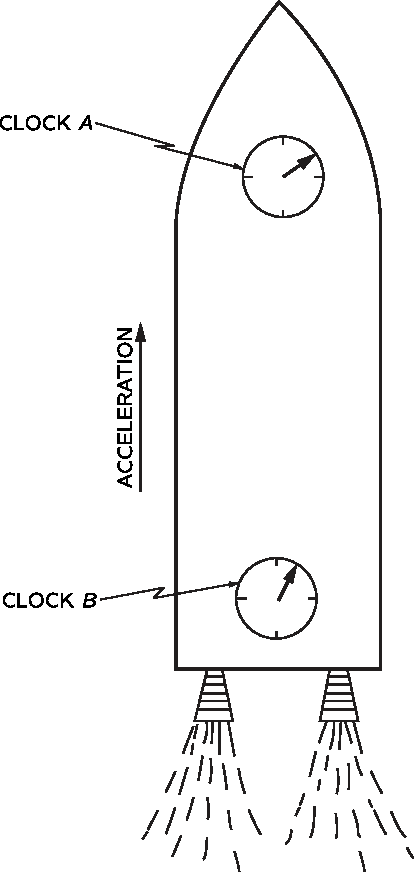
\includegraphics[width=0.5\linewidth]{fyz_fig531.pdf}
      \caption{Zrychlující se raketa se dvěma hodinami (\cite[s.~786]{Feynman02})}
      \label{fyz:fig531}
    \end{figure}
    
    První záblesk projde vzdálenost \(L_1\), zatímco druhý kratší vzdálenost \(L_2\). Vzdálenost je 
    kratší, neboť raketa se zrychluje a v okamžiku druhého záblesku má vyšší rychlost. Vidíme, že 
    pokud byly oba záblesky z hodin \(A\) vyslány s jednosekundovým časovým posunem, dojdou k 
    hodinám \(B\) oddělené intervalem kratším než sekunda, neboť druhý záblesk na cestě stráví 
    kratší dobu.
    
    Totéž se bude dít s pozdějšími záblesky. Kdybychom tedy seděli v ocasu, dospěli bychom k 
    závěru, že hodiny \(A\) běží rychleji než \(B\). Pokud bychom provedli celou věc naopak, 
    nechali hodiny \(B\) vysílat světlo a pozorovali jej u hodin \(A\), zdálo by se vám, že hodiny 
    \(B\) běží \emph{pomaleji} než \(A\). Vše souhlasí a není na tom nic záhadného.
    
    Nyní si představme, že raketa je v klidu na zemském povrchu. \emph{Děje se totéž}. Sedíme-li s 
    jedněmi hodinami na podlaze a pozorujeme druhé, které leží na vysoké poličce, zdá se, že běží 
    rychleji než hodiny na podlaze! Řekneme: „To není správně. Časy musí být stejné. V případě bez 
    zrychlení není důvod proč by hodiny neměly jít stejně.“ Musí to však tak být, platí-li princip 
    ekvivalence. Einstein trval na tom, že princip je správný a postupoval odvážně vpřed. 
    Prohlásil, že hodiny na různých místech v gravitačním poli musí zdánlivě jít různými 
    rychlostmi. Jdou-li však vždy \emph{zdánlivě} vzhledem k sobě různou rychlostí, pak vzhledem k 
    prvním hodinám druhé opravdu jinou rychlostí jdou.
    
    Teď vidíme, že tu máme s hodinami analogickou situaci jako se zahřátým pravítkem, o kterém jsme 
    mluvili dříve, když jsme si všímali brouka na zahřáté desce. Představovali jsme si, že pravítka 
    i brouci a vůbec vše se měnilo stejným způsobem při změně teploty, takže brouci nikdy nemohli 
    zjistit, že jejich měřicí pomůcky se změnily při pohybu po ohřáté desce. Podobné je to v 
    případě hodin v gravitačním poli. Každé hodiny, které umístíme na vyšší úroveň, běží viditelně 
    rychleji. Tlukot srdce je rychlejší, všechny procesy probíhají rychleji.

    \begin{figure}[ht!] %\ref{fyz:fig532}
      \centering
      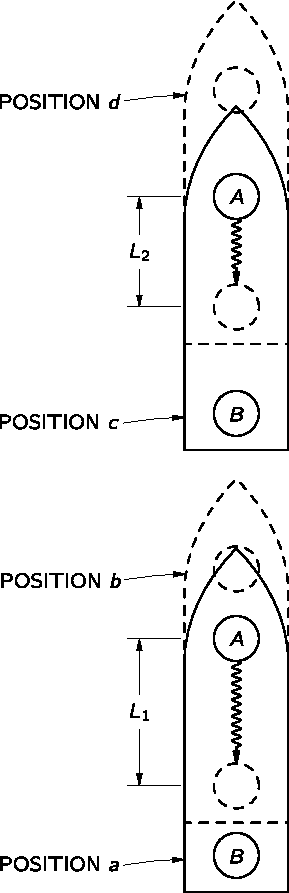
\includegraphics[width=0.5\linewidth]{fyz_fig532.pdf}
      \caption{Hodiny v přední části zrychlující rakety běží zdánlivě rychleji než hodiny v zadní 
               části. (\cite[s.~787]{Feynman02})}
      \label{fyz:fig532}
    \end{figure}
    
    Pokud by to tak nebylo, mohli bychom odlišit gravitační pole od zrychlující vztažné soustavy. 
    Představa, že čas se může od místa k místu měnit, není jednoduchá, ale právě tuto představu 
    Einstein použil, a - věřte nebo nevěřte - je správná.
    
    Pomocí principu ekvivalence můžeme vypočítat, jak se mění rychlost hodin v gravitačním poli s 
    výškou. Stačí vypočítat zdánlivou odchylku mezi dvěma hodinami ve zrychlující se raketě. 
    Nejsnáze to můžeme provést pomocí výsledku pro Dopplerův jev, který jsme odvodili v kapitole 
    \ref{fyz:IchapXXXIV} dílu \ref{part:FYZI}. Tam jsme zjistili (viz vztah (\ref{fyz:eq531})), že 
    je-li \(v\) \emph{relativní} rychlost zdroje a přijímače, souvisí \emph{zachycená} frekvence 
    \(\omega\) s \emph{vyslanou} frekvencí \(\omega_0\) podle vztahu
    \begin{equation}\label{fyz:eq532}
      \omega = \omega_0\dfrac{1+\dfrac{v}{c}}{\sqrt{1-\dfrac{v^2}{c^2}}}.
    \end{equation}
    Zamyslíme-li se nyní nad zrychlující se raketou na obr. \ref{fyz:fig532}, vidíme, že vysílač i 
    přijímač se pohybují v každém okamžiku stejnými rychlostmi. Ale za čas, za který projde 
    světelný signál od hodin \(A\) k \(B\), se raketa zrychlila. Ve skutečnosti nabyla dodatečnou 
    rychlost \(gt\), přičemž \(g\) je zrychlení a \(t\) je čas, za který světlo urazí vzdálenost 
    \(H\) z \(A\) do \(B\). Tento čas je velmi blízký \(H/c\). 
    
    Dojde-li tedy signál k \(B\), zvýšila raketa svou rychlost o \(gH/c\). Přijímač má takovou 
    rychlost vždy vůči rychlosti vysílače v okamžiku, kdy ho signál opustil. To je tedy rychlost, 
    kterou musíme dosadit do vztahu (\ref{fyz:eq532}) pro Dopplerův posun. Předpokládáme-li, že 
    zrychlení a délka kosmické lodi jsou dostatečně malé, takže tato rychlost je mnohem menší než 
    \(c\), můžeme zanedbat členy řádu \(v^2/c^2\). Vyjde nám
    \begin{equation}\label{fyz:eq533}
      \omega = \omega_0\left(1 + \dfrac{gH}{c^2}\right).
    \end{equation}
    
    V případě dvou hodin v raketě platí vztah
    \begin{equation*}
      \binom{\text{frekvence hodin}}{\text{příjímače}} 
        = \binom{\text{frekvence hodin}}{\text{vysílače}}\cdot\left(1 + \dfrac{gH}{c^2}\right)
    \end{equation*}
    přičemž \(H\) je výška vysílače nad přijímačem. 
    
    \emph{Na základě principu ekvivalence musí platit stejný vztah v případě dvojích hodin 
    oddělených výškovým rozdílem \(H\) v gravitačním poli se zrychlením volného pádu} \(g\). 
    
    To je natolik důležitá myšlenka, že bychom vám chtěli dokázat, že vyplývá i z jiného zákona 
    fyziky - ze zákona zachování energie. Víme, že gravitační síla, která působí na těleso, je 
    úměrná její hmotnosti \(M\), která je ve vztahu k celkové vnitřní energii \(E\). \(M=E/c^2\). 
    Například hmotnosti jader určené z energií jaderných reakcí, při nichž dochází k přeměně jader, 
    souhlasí s hmotnostmi získanými z \emph{atomových hmotností}.
    
    Nyní si představme atom, jehož nejnižší energetický stav má celkovou energii \(E_0\) a vyšší 
    stav energii \(E_1\) a který může přejít ze stavu \(E_1\) do stavu \(E_0\), emitováním světla. 
    Frekvence \(\omega\) tohoto světla bude dána vztahem
    \begin{equation}\label{fyz:eq534}
      \hbar\omega = E_1 - E_0.
    \end{equation}
    
    Nechť je takový atom původně na podlaze a přeneseme jej odtud do výšky \(H\). Musíme přitom 
    vykonat práci, která je potřebná k přesunu hmotnosti \(m_1 = E_1/c^2\) proti směru působení 
    gravitační síly. Vykonaná práce je
    \begin{equation}\label{fyz:eq535}
      \dfrac{E_1}{c^2}gH.
    \end{equation}
    
    Pak necháme atom vyslat foton a přejít do nižšího energetického stavu \(E_0\). Poté atom 
    přeneseme zpět na podlahu. Při návratu je hmotnost \(E_0/c^2\); zpět získáme energii
    \begin{equation}\label{fyz:eq536}
      \dfrac{E_0}{c^2}gH,
    \end{equation}
    takže jsme vykonali celkovou práci
    \begin{equation}\label{fyz:eq537}
      \Delta W = \dfrac{E_1 - E_0}{c^2}gH.
    \end{equation}
    
    Když atom emitoval foton, odevzdal energii \(E_1 - E_0\). Představme si, že se foton náhodou 
    vrátil na podlahu a byl absorbován. Kolik energie by odevzdal? V prvním okamžiku bychom si 
    mohli myslet, že by odevzdal energii \(E_1 - E_0\). To však nemůže být pravda, zachovává-li se 
    energie. Na začátku jsme měli energii \(E_1\) na podlaze. Na konci je energie na úrovni podlahy 
    součtem energie \(E_0\) atomu v nižším stavu a energie \(E_{tot}\) absorbovaného fotonu. Mezi 
    tím jsme však museli dodat dodatečnou energii \(\Delta W\) podle vztahu (\ref{fyz:eq537}). 
    Zachovává-li se energie, musí být energie, s níž skončíme na podlaze, větší než počáteční 
    energie o hodnotu vykonané práce. Musí platit
    \begin{subequations}
      \begin{align}
        E_{fot} + E_0 = E_1 + \Delta W       \label{fyz:eq538a}  \\
        \shortintertext{neboli}
        E_{fot} = E_1 - E_1 + \Delta W.      \label{fyz:eq538b}
      \end{align}
    \end{subequations}

    Musí to být tak, že foton na úroveň podlahy \emph{nedopadne} jen s energií \(E_1 - E_0\) s níž 
    byl vyslán, ale s \emph{o něco větší energií}. Jinak by se nějaká energie ztratila. Dosadíme-li 
    do rovnice (\ref{fyz:eq538b}) \(\Delta W\) z rovnice (\ref{fyz:eq537}), vyjde nám, že foton 
    dopadne na úroveň podlahy s energií
    \begin{equation}\label{fyz:eq539}
      E_{fot} = (E_1-E_0)\left(1 + \dfrac{gH}{c^2}\right).
    \end{equation}
    
    Ale foton s energií \(E_{fot}\) má frekvenci \(\omega = E_{fot}/\hbar\). Označíme-li frekvenci 
    \emph{vyslaného} fotonu \(\omega_0\) (musí být podle (\ref{fyz:eq534}) rovna \((E_1 — 
    E_0)\hbar\)), náš výsledek (\ref{fyz:eq539}) vede opět ke vztahu (\ref{fyz:eq533}) mezi 
    frekvencí fotonu absorbovaného na podlaze a frekvencí s jakou byl vyslán.
    
    Stejný výsledek můžeme získat ještě jinak. Foton s frekvencí \(\omega_0\) má energii \(E = 
    \hbar\omega_0\). Jelikož energii \(E_0\) odpovídá gravitační hmotnost \(E_0/c^2\), má foton 
    hmotnost (ne klidovou hmotnost!) \(\hbar\omega_0/c^2\) a je „přitahován“ k Zemi. Při pádu z 
    výšky \(H\) získá  dodatečnou energii \((\hbar\omega_0/c^2)gH\), takže dopadne s energií
    \begin{equation*}
      E = \hbar\omega_0\left(1 + \dfrac{gH}{c^2}\right).
    \end{equation*}
    Jeho frekvence po pádu je \(E/\hbar\), což opět vede k výsledku (\ref{fyz:eq533}). Naše 
    představy o relativitě, kvantové fyzice a zachování energie navzájem souhlasí pouze tehdy, 
    jsou-li Einsteinovy předpovědi o hodinách v gravitačním poli správné. Změny frekvence, o nichž 
    hovoříme, jsou obvykle velmi malé. Například při rozdílu výšek \num{20} metrů u zemského 
    povrchu je rozdíl frekvencí přibližně jen \num{2e-15}. Právě takovou změnu se však podařilo 
    experimentálně změřit pomocí \textbf{Mössbauerova jevu}. Einstein měl úplnou pravdu.
    
  \section{Křivost časoprostoru}\label{fyz:IIchapXVLIIsecVII}
    Nyní bychom chtěli vše, o čem jsme hovořili, dát do souvislosti s představou o zakřiveném 
    časoprostoru. Už jsme poznamenali, že běží-li čas různými rychlostmi na různých místech, je to 
    analogické se zakřiveným prostorem ohřáté desky. Je to však víc než analogie; znamená to, že 
    časoprostor je opravdu zakřiven. Pokusme se o trochu geometrie v časoprostoru. Na první pohled 
    to může vypadat zvláštně, ale vždyť jsme už mnohokrát kreslili časoprostorové diagramy se 
    vzdálenostmi nanesenými na jednu osu a časem na druhou. Zkusme vytvořit pravoúhelník v 
    časoprostoru. Nejprve nakreslíme graf výšky \(Hv\) závislosti na čase \(t\) jako na obr. 
    \ref{fyz:fig533a}. Abychom vytvořili základnu našeho pravoúhelníku, vezmeme si předmět, který 
    je \emph{v klidu} ve výšce a budeme sledovat jeho světočáru \num{100} sekund. Získáme tak 
    úsečku \(BDv\) části \(b\) obrázku, která je rovnoběžná s osou \(t\). Nyní si vezmeme další 
    předmět, který je v čase \(t = 0\) \num{100} metrů nad prvním. Vyjde z bodu \(A\) na obr. 
    \ref{fyz:fig533c}. Nyní sledujme jeho světočáru po dobu \num{100} sekund, kterou měříme pomocí 
    hodin v bodě \(A\). Předmět projde z bodu \(A\) do \(C\) jak znázorňuje část \(d\) obrázku. 
    Všimněme si však, že v důsledku toho, že hodiny v různých výškách jdou různou rychlostí 
    (předpokládáme přítomnost gravitačního pole), body \(C\) a \(D\) nejsou současné. Pokusíme-li 
    se doplnit pravoúhelník úsečkou do bodu \(C\), který leží \num{100} metrů nad bodem \(D\) ve 
    stejném čase (obr. \ref{fyz:fig533e}) obrazec se neuzavře. Právě toto máme na mysli, když 
    říkáme, že časoprostor je zakřiven.
    
    \begin{figure}[ht!] %\ref{fyz:fig533}
      \centering  
      \subcaptionbox{\label{fyz:fig533a}}{\luafigure[0.70]{fyz_fig533a.pdf}}    \\
      \subcaptionbox{\label{fyz:fig533b}}{\luafigure[0.70]{fyz_fig533b.pdf}}    \\
      \subcaptionbox{\label{fyz:fig533c}}{\luafigure[0.70]{fyz_fig533c.pdf}}    \\
      \subcaptionbox{\label{fyz:fig533d}}{\luafigure[0.70]{fyz_fig533d.pdf}}    \\
      \subcaptionbox{\label{fyz:fig533e}}{\luafigure[0.70]{fyz_fig533e.pdf}}            
      \caption{Pokus vytvořit pravoúhelník v časoprostoru (\cite[s.~790]{Feynman02}).}
      \label{fyz:fig533}
    \end{figure}     

  \section{Pohyb v zakřiveném časoprostoru}\label{fyz:IIchapXVLIIsecVIII}
    Podívejme se na zajímavou hádanku. Máme dvojici identických hodin, \(A\) a \(B\), které leží na 
    povrchu Země jako na obr. \ref{fyz:fig534}. Zvedneme hodiny \(A\) do nějaké výšky \(H\), chvíli 
    je tam podržíme a opět vrátíme na Zem, právě ve chvíli, kdy druhé hodiny \(B\) ušli o \num{100} 
    sekund. Hodiny \(A\) ukáží řekněme \num{107} sekund, neboť nahoře ve vzduchu běžely rychleji. 
    Tady je naše hádanka: Jak máme pohybovat hodinami \(A\) aby ukazovaly co nejvyšší hodnotu 
    uplynulého času, za předpokladu, že se vrátí, když hodiny \(B\) ukazují \num{100} sekund? 
    Řekneme si: „To je snadné. Jednoduše zvedneme hodiny \(A\) co nejvýše. Tam poběží nejrychleji, 
    tudíž uplyne nejvíce času, než se vrátí.“ To je ale chyba. Na něco jste zapomněli - na cestu 
    vzhůru a dolů máme jen \num{100} sekund. Vyrazíme-li velmi vysoko, musíme se vrátit velmi 
    rychle, abychom prošli tam a zpět za \num{100} sekund. A nesmíme zapomenou na efekt speciální 
    relativity, který způsobuje, že se pohybující hodiny \emph{zpomalí} \(\sqrt{V1 - 
    v2/c^2}\)-krát. Tento relativistický jev způsobuje, že hodiny \(A\) ukazují \emph{menší} čas 
    než hodiny \(B\). Vidíme, že tu máme zajímavou hru.
    
    \begin{figure}[ht!] %\ref{fyz:fig534}
      \centering
      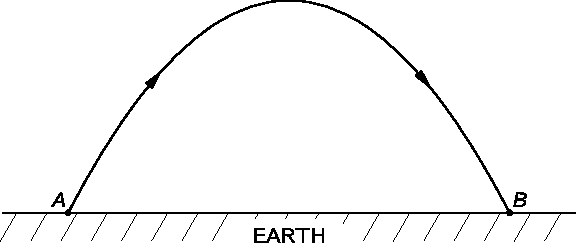
\includegraphics[width=0.9\linewidth]{fyz_fig534.pdf}
      \caption{V homogenním gravitačním poli je trajektorie s maximálním vlastním časem při dané 
               hodnotě uplynulého času parabola
               (\cite[s.~791]{Feynman02})}
      \label{fyz:fig534}
    \end{figure}
    
    Nebudeme-li hodinami \(A\) hýbat, dostaneme \num{100} sekund. Přesuneme-li je do malé výšky a 
    pomalu se vrátíme, získáme o trochu více než \num{100} sekund. Posuneme-li je o kousek výše, 
    získáme možná ještě o trochu víc. Posuneme-li je příliš vysoko, musíme se pohybovat rychle, a 
    tak zpomalit naše hodiny na tolik, že se vrátíme s méně než \num{100} sekundami. Jaký jízdní 
    řád, jaká závislost výšky na čase, nám dá nejvyšší možnou hodnotu na hodinách \(A\)? Jak vysoko 
    se máme posunout, jakou pečlivě vybranou rychlostí se tam máme dostat, abychom se k hodinám 
    \(B\) vrátili právě v okamžiku, kdy na nich uplyne \num{100} sekund?
    
    Odpověď je následující. Vypočítejme, jak rychle musíme vyhodit míč směrem vzhůru do vzduchu, 
    aby na zem dopadl přesně za \num{100} sekund. Pohyb míče – nejprve rychlý vzestup, zpomalení, 
    zastavení a zpětný návrat na zem - jsou tím pravým pohybem, který maximalizuje čas, který 
    uplyne na hodinách připevněných k míči.
    
    Nyní si všimněme trochu jiného problému. Mějme dva body \(A\) a \(B\) na zemském povrchu v 
    nějaké vzdálenosti od sebe. Zahrajme si stejnou hru, jako když jsme hledali „úsečku“. Ptáme se, 
    jak se máme přesunout z \(A\) do \(B\), aby čas na našich pohybujících se hodinách byl co 
    největší. Předpokládáme, že z \(A\) vyrazíme na daný signál a do \(B\) dojdeme současně s jiným 
    signálem, o němž podle nehybných hodin víme, že je posunut o \num{100} sekund. Nyní řekneme: 
    „Vždyť jsme zjistili, že je třeba se pohybovat po přímce konstantní rychlostí zvolenou tak, 
    abychom do \(B\) dorazili přesně o \num{100} sekund později. Nebudeme-li se pohybovat po 
    přímce, budeme muset jít vyšší rychlostí a to zpomalí naše hodiny."
    
    Ale počkejme. Tehdy jsme nebrali v úvahu gravitaci. Není lepší se pohybovat chvíli vzhůru po 
    zakřivené dráze a pak klesat dolů? Tak strávíme část času ve výšce, kde naše hodiny poběží 
    rychleji. Opravdu je tomu tak. Vyřešíme-li matematickou úlohu, jak zvolit křivku pohybu tak, 
    aby čas, který uplyne na pohybujících se hodinách, byl co největší, zjistíte, že pohyb probíhá 
    po \emph{parabole} - po téže křivce, po níž se pohybuje těleso při šikmém vrhu v gravitačním 
    poli (obr. \ref{fyz:fig534}). Proto můžeme zákon pohybu v gravitačním poli formulovat i takto: 
    \textbf{Těleso se vždy pohybuje z místa na místo po takové trajektorii, že hodiny s ním spojené 
    ukazují delší čas, než na kterékoliv jiné možné trajektorii}, samozřejmě, při stejných 
    počátečních a konečných podmínkách. Čas, který měří pohybující se hodiny, se často nazývá 
    jejich vlastním časem. Při volném pádu trajektorie maximalizuje vlastní čas tělesa. 

    Podívejme se, jak se k tomu všemu dojde. Vyjdeme z rovnice (\ref{fyz:eq533}), která říká, že 
    nadbytečná rychlost chodu pohybujících se hodin je    
    \begin{equation}\label{fyz:eq540}
      \dfrac{\omega_0gH}{c^2}.
    \end{equation}
    Kromě toho si musíme pamatovat, že existuje i korekce opačného znaménka v důsledku rychlosti. U 
    tohoto jevu víme, že    
    \begin{equation*}
      \omega = \omega_0\sqrt{1 - \dfrac{v^2}{c^2}}.
    \end{equation*}
    Ačkoliv zákon platí pro libovolnou rychlost, všimneme si případu, kdy jsou rychlosti mnohem 
    menší než \(c\). Pak můžeme rovnici zapsat jako
    \begin{equation*}
      \omega = \omega_0\left(1 - \dfrac{v^2}{2c^2}\right).
    \end{equation*}
    a úbytek rychlosti chodu hodin je
    \begin{equation}\label{fyz:eq541}
      -\omega_0\dfrac{v^2}{2c^2}.
    \end{equation}
    Složíme-li oba členy \ref{fyz:eq540} a \ref{fyz:eq541}, zjistíme že 
    \begin{equation}\label{fyz:eq542}
      \Delta\omega = \dfrac{\omega_0}{c^2}\left(gH - \dfrac{v^2}{2}\right).
    \end{equation}
    Takový posun frekvence našich pohybujících se hodin znamená, že změříme-li čas \(\dd{t}\) na 
    nehybných hodinách, hodiny v pohybu zaznamenají čas
    \begin{equation}\label{fyz:eq543}
     \dd{t}\left[1 + \left(\dfrac{gH}{c^2} - \dfrac{v^2}{2c^2}\right)\right].
    \end{equation}
    Celkový přírůstek času podél trajektorie je integrálem nadbytečného členu podle času, tj.
    \begin{equation}\label{fyz:eq544}
      \dfrac{1}{c^2}\int\left(gH - \frac{v^2}{2}\right)\dd{t},
    \end{equation}

    a ten má být maximální. Člen \(gH\) je právě gravitační potenciál \(\varPhi\). Celou rovnici 
    vynásobíme konstantou - \(mc^2\), přičemž \(m\) je hmotnost tělesa. Konstanta nezmění podmínku 
    maxima a záporné znaménko změní jen maximum na minimum. Rovnice (\ref{fyz:eq544}) pak říká, že 
    těleso se bude pohybovat tak, aby
    \begin{equation}\label{fyz:eq545}
      \int\left(\dfrac{mv^2}{2} - m\varphi\right)\dd{t} = \text{minimum}.
    \end{equation}
    Pod integrálem je právě rozdíl kinetické a potenciální energie. Podíváme-li se do kapitoly
    \ref{fyz:IIchapXIX}, uvidíme, že při diskuzi principu nejmenšího účinku jsme ukázali, že
    Newtonovy zákony pro těleso v poli potenciálu lze zapsat přesně ve tvaru rovnice
    (\ref{fyz:eq545}).
    
  \section{Einsteinova teorie gravitace}\label{fyz:IIchapXVLIIsecIX}
    Einsteinův tvar pohybových rovnic - požadavek, že vlastní čas má být v zakřiveném časoprostoru 
    maximální-vede při nízkých rychlostech ke stejným výsledkům jako Newtonovy zákony. Při obězích 
    kolem Země ukazovaly hodinky Gordona Coopera delší čas, než na jakékoliv jiné dráze, kterou 
    byste si pro jeho družici dokázali představit\footnote{Přesněji je to jen lokální maximum, 
    Raději bychom měli říci, že vlastní čas je větší než na jakékoliv blízké trajektorii. Například 
    vlastní čas na eliptické dráze kolem Země nemusí být delší než na balistické dráze tělesa, 
    které je vystřeleno do velké výšky a pak padá zpět.}.
    
    Zákon gravitace lze tedy pomocí geometrické představy o časoprostoru vyjádřit tímto 
    pozoruhodným způsobem: Částice si při pohybu vyberou nejdelší vlastní čas, což je veličina, 
    která je v časoprostoru analogem „nejkratší vzdálenosti“. Takový je zákon pohybu v gravitačním 
    poli. Velkou výhodou takové formulace je, že nezávisí na žádných souřadnicích ani jiném způsobu 
    specifikace situace.
    
    Shrňme, co jsme už udělali. Zformulovali jsme dva zákony gravitace:
    \begin{itemize}
      \item Jak se mění geometrie časoprostoru v přítomnosti hmoty: křivost vyjádřená pomocí 
            nadbytečného poloměru je úměrná hmotnosti uvnitř koule (viz vztah (\ref{fyz:eq530})).
      \item Jak se tělesa pohybují, působí-li jen gravitační síly: pohybují se tak, aby vlastní čas 
             mezi oběma krajními body dráhy byl maximální.
    \end{itemize}
    
    Tyto dva zákony odpovídají podobným párům rovnic, s nimiž jsme se setkali dříve. Původně jsme 
    pohyb v gravitačním poli popsali pomocí Newtonova gravitačního zákona („zákonu převráceného 
    čtverce") a jeho pohybových rovnic. Zákony \num{1} a \num{2} nyní zaujaly jejich místo. Náš 
    nový pár rovnic odpovídá také tomu, co jsme viděli v elektrodynamice. Tam jsme měli zákon, 
    soustavu Maxwellových rovnic, která určuje pole vytvářená náboji. Říká nám, jak se „prostor“ 
    změní v důsledku přítomnosti nabitých částic; plní podobnou úlohu jako zákon 1 v gravitaci. 
    Navíc jsme měli zákon pohybu částic v daných polích - \(d(m\vec{v})/dt = g(\vec{E} + 
    \vec{v}\times\vec{B})\). Tuto úlohu v gravitaci hraje zákon \num{2}.
    
    V zákonech \num{1} a \num{2} máme přesnou formulaci \emph{Einsteinovy teorie gravitace} - 
    ačkoliv ji obvykle najdeme zformulovanou v komplikovanějším matematickém tvaru. Měli bychom 
    však ještě něco přidat. Podobně jako se časová měřidla v gravitačním poli mění od místa k 
    místu, mění se i měřidla délky. Pravítka mění při pohybu svou délku. Jsou-li prostor a čas tak 
    úzce svázány, není možné, aby se s časem dělo něco, coby se nějak neodráželo i v prostoru. 
    Vezměme si nejjednodušší případ: Prolétáváme kolem Země. Co je \emph{čas} z \emph{vašeho} 
    hlediska, je z části prostor z \emph{našeho} hlediska. Musí tedy docházet ke změnám v prostoru. 
    Celý \emph{časoprostor} je přítomností hmoty zakřiven, a to je složitější situace než pouhá 
    změna časové škály. Pravidlo, které jsme uvedli ve vztahu (\ref{fyz:eq530}), však postačuje k 
    úplnému určení všech zákonů gravitace, je-li chápáno v tom smyslu, že toto pravidlo o křivosti 
    neplatí jen z hlediska jednoho pozorovatele, ale platí obecně. Někdo, kdo prochází množstvím 
    látky, vidí jiný obsah hmoty v důsledku kinetické energie svého pohybu; musí zahrnout hmotnost, 
    která této energii odpovídá. Teorie musí být vytvořena tak, aby každý - bez ohledu na to, jak 
    se pohybuje - zjistil, že nadbytečný poloměr nějaké kouleje \(\varkappa/3c^2\) krát celková 
    hmotnost (nebo lépe \(\varkappa/3c^4\) krát celkový obsah energie) uvnitř koule. To, že tento 
    zákon - zákon \num{1} - musí platit v libovolné pohybující se soustavě, je jedním z velkých 
    zákonů gravitace, který se nazývá \textbf{Einsteinova rovnice pole}. Druhý velký zákon \num{2} 
    (tj., že věci se musí pohybovat tak, aby vlastní čas byl maximální) se nazývá 
    \textbf{Einsteinova rovnice pohybu}. 
    
    Zapsat tyto rovnice v úplném algebraickém tvaru, porovnat je s Newtonovy zákony a dát je do 
    souvislosti s elektrodynamikou je matematicky obtížné. Ale právě tak dnes vypadají nejúplnější 
    zákony fyziky gravitace. 
    
    Ačkoliv nám v jednoduchém případě, který jsme zkoumali, poskytly výsledek ve shodě s Newtonovou 
    mechanikou, není to tak vždycky. Tři odchylky, které Einstein jako první odvodil, byly 
    potvrzeny experimentálně: 
    \begin{enumerate}
      \item dráha Merkuru není nehybná elipsa;
      \item světlo hvězdy se při průchodu v blízkosti Slunce ohýbá dvakrát více, než bychom 
            očekávali
      \item rychlost hodin v gravitačním poli závisí na jejich poloze.
    \end{enumerate}
    Kdykoliv se Einsteinovy předpovědi odlišily od představ Newtonovy mechaniky, příroda si volila 
    Einsteina. 
    
    Nakonec shrňme vše, co jsme řekli, takto: Za prvé, měřidel času a délky závisí na místě v 
    prostoru, kde je měříme, a na čase. To je ekvivalentní s tvrzením, že časoprostor je zakřiven. 
    Z naměřené velikosti povrchu koule můžeme definovat její očekávaný poloměr, \(\sqrt{S/4\pi}\), 
    ale skutečný naměřený poloměr bude větší o hodnotu, která je úměrná (konstanta úměrnosti je 
    \(\varkappa/3c^2\)) celkové hmotnosti, obsažené uvnitř koule. To přesně určuje stupeň zakřivení 
    našeho časoprostoru. Křivost musí být stejná bez ohledu na to, kdo se dívá na hmotu, nebo jak 
    se pohybuje. Za druhé, částice se pohybují v tomto zakřiveném časoprostoru po „úsečkách“ (po 
    trajektoriích s maximálním vlastním časem). To je obsah Einsteinovy formulace zákonů gravitace.